% =========================================================================
% Stato dei lavori (Web Science 2027): traccia viva di cosa e' stato fatto
% e di cosa faremo. Nata dalla parte "Esperimenti di John" della riunione
% dopo IrForGood (Riunioni/Riunione dopo IrForGood), poi staccata.
% Figure: figure/genera_figure.py (legge Code/WebScience2027).
% Build: tectonic stato_dei_lavori.tex
% =========================================================================
\documentclass[aspectratio=169]{beamer}
\usetheme{Madrid}
\usecolortheme{whale}
\usepackage[T1]{fontenc}
\usepackage{graphicx}
\usepackage{booktabs}
\usepackage{xcolor}
\usepackage{tikz}
\graphicspath{{./figure/}{./}}

\beamertemplatenavigationsymbolsempty
\setbeamercovered{invisible}
\setbeamertemplate{caption}{\insertcaption}
\newcommand{\hl}[1]{\textbf{#1}}
\newenvironment{johnblock}{\begin{exampleblock}{\footnotesize Commento di John}\footnotesize}{\end{exampleblock}}
\newenvironment{claudeblock}{\setbeamercolor{block title}{fg=white,bg=gray!65!black}\setbeamercolor{block body}{bg=gray!12}\begin{block}{\footnotesize Commento di Claude}\footnotesize}{\end{block}}
\newcommand{\divider}[2]{%
  \begin{frame}[plain]
    \vfill
    \begin{center}
      {\color{dividerblue}\Huge\textbf{#1}}\\[0.8em]
      {\large #2}
    \end{center}
    \vfill
  \end{frame}}
\definecolor{wrongred}{RGB}{176,0,32}
\definecolor{dividerblue}{RGB}{28,42,92}
\newcommand{\wrong}[1]{\textcolor{wrongred}{#1}}

\title[Stato dei lavori]{Stato dei lavori}
\subtitle{Web Science 2027: cosa abbiamo fatto e cosa faremo}
\author[John Bianchi]{John Bianchi}
\institute[]{IMT Lucca \& IIT-CNR Pisa}
\date{}

\begin{document}

\begin{frame}
  \titlepage
\end{frame}

% ===================================================================================================
\divider{Il primo dataset}{dai transformer del paper a un classificatore pi\`u semplice}

\begin{frame}{Il punto di partenza: i transformer del paper}
  \vfill
  \begin{itemize}[<+->]
    \setlength\itemsep{0.8em}
    \item Il dataset di IrForGood: \hl{439 testate}, \hl{19.476 articoli}; 5 fold, nel test solo testate \hl{mai viste} in addestramento
    \item \hl{Per articolo}: accuratezza intorno a \hl{0,60} (da 0,58 di BERT a 0,61 di Mistral), F1 macro 0,52--0,55
    \item \hl{Per testata} (voto di maggioranza dei suoi articoli): accuratezza fino a \hl{0,69} (RoBERTa; Mistral 0,68), tolerant 1 fino a 0,88
    \item[] {\small\itshape Modelli da 110 milioni a 24 miliardi di parametri, tutti pi\`u o meno allo stesso livello.}
  \end{itemize}
  \vfill
\end{frame}

\begin{frame}{Un classificatore a feature fa lo stesso, se non meglio}
  \begin{itemize}[<+->]
    \setlength\itemsep{0.5em}
    \item \hl{TF-IDF}: ogni articolo diventa l'elenco delle sue parole (e coppie di parole), pesate per quanto sono rare; sopra, una \hl{regressione logistica}. Nessuna rete neurale: si addestra in un minuto
    \item Sugli \hl{stessi fold} del paper:
  \end{itemize}
  \vspace{0.3em}
  \visible<3->{%
  \centering\small
  \begin{tabular}{lcccc}
    \toprule
    & \multicolumn{2}{c}{\textbf{per articolo}} & \multicolumn{2}{c}{\textbf{per testata}} \\
    \cmidrule(lr){2-3}\cmidrule(lr){4-5}
    & accuratezza & F1 macro & accuratezza & tolerant 1 \\
    \midrule
    migliore dei 4 transformer (misura per misura) & 0,61 & 0,55 & 0,69 & 0,88 \\
    \textbf{TF-IDF + regressione logistica} & 0,58 & 0,52 & \textbf{0,68} & \textbf{0,88} \\
    \bottomrule
  \end{tabular}\par}
  \vspace{0.6em}
  \begin{itemize}[<+->]
    \setcounter{beamerpauses}{4}
    \item Come fa un modello che \hl{conta parole} ad andare come Mistral da 24 miliardi di parametri?
    \item Per capirlo ho guardato \hl{dentro il dataset}
  \end{itemize}
\end{frame}

\begin{frame}{Quanto si somigliano due articoli? (1) I pezzetti di 5 parole}
  \begin{itemize}[<+->]
    \setlength\itemsep{0.6em}
    \item Il testo si \hl{normalizza}: minuscole, niente punteggiatura, i numeri diventano \#
    \item Poi si spezza in tutti i \hl{pezzetti di 5 parole consecutive}:
    \item[] {\small\ttfamily there was a single gas station in cities across phillips county}\\[0.2em]
            {\small $\to$ \ttfamily [there was a single gas] [was a single gas station] [a single gas station in] \dots}
    \item \hl{Somiglianza di Jaccard} tra due articoli $A$ e $B$:
    \[ J(A,B) = \frac{\text{pezzetti in comune}}{\text{pezzetti di tutti e due, contati una volta}} = \frac{|A \cap B|}{|A \cup B|} \]
    \item $J = 0$: niente in comune; $J = 1$: lo stesso testo. \hl{$J \geq 0{,}5$}: pi\`u di met\`a dei pezzetti in comune, gli articoli sono \hl{quasi uguali} (non per forza identici)
  \end{itemize}
\end{frame}

\begin{frame}{Quanto si somigliano due articoli? (2) Un esempio vero}
  \begin{columns}[t]
    \begin{column}{0.48\textwidth}
      \begin{block}{\footnotesize ncindiananews.com}
        \scriptsize Federal Energy Regulatory Commission (FERC) Commissioner Mark C. Christie \textbar{} www.ferc.gov\\[0.3em]
        There was a single gas station in cities across \hl{White County} selling premium gas at the lowest price of \hl{\$3.81} per gallon \dots
      \end{block}
    \end{column}
    \begin{column}{0.48\textwidth}
      \begin{block}{\footnotesize savannahstandard.com}
        \scriptsize Federal Energy Regulatory Commission (FERC) Commissioner Mark C. Christie \textbar{} www.ferc.gov\\[0.3em]
        There were two gas stations in cities across \hl{Bulloch County} selling premium gas at the lowest price of \hl{\$3.79} per gallon \dots
      \end{block}
    \end{column}
  \end{columns}
  \vspace{0.6em}
  \begin{itemize}[<+->]
    \setlength\itemsep{0.5em}
    \item Due siti diversi, lo \hl{stesso articolo-modello}: cambiano solo la contea e i numeri
    \item Sono articoli \hl{generati in serie} da una rete di siti locali: il testo \`e quasi tutto uguale ($J$ tra 0,6 e 1)
    \item Un classificatore che ha visto uno di questi nel training riconosce subito l'altro nel test
  \end{itemize}
\end{frame}

\begin{frame}{Quanto si somigliano due articoli? (3) Confrontarli tutti}
  \vfill
  \begin{itemize}[<+->]
    \setlength\itemsep{0.8em}
    \item 19.476 articoli sono quasi \hl{190 milioni di coppie}: calcolare $J$ esatto su tutte, testo contro testo, \`e \hl{impossibile} in tempi ragionevoli
    \item \hl{MinHash} e \hl{LSH} servono a questo: calcolano la somiglianza di Jaccard in modo \hl{fattibile}, accettando una piccola \hl{approssimazione}
    \item[] MinHash riassume ogni articolo in un'\hl{impronta} corta da cui si stima $J$; LSH propone solo le coppie che \hl{probabilmente} si somigliano
    \item[] {\small\itshape \`E la tecnica standard per togliere i duplicati dai dati di addestramento dei modelli linguistici.}
    \item Risultato: \hl{1.557} articoli hanno una copia \hl{identica} su un'altra testata; \hl{4.740} (il \hl{24\%}) una copia \hl{quasi uguale} ($J \geq 0{,}5$)
  \end{itemize}
  \vfill
\end{frame}

\begin{frame}{Dagli articoli alle reti di testate}
  \begin{columns}[c]
    \begin{column}{0.42\textwidth}
      \begin{itemize}[<+->]
        \setlength\itemsep{0.6em}
        \item Due testate sono \hl{collegate} se hanno \hl{almeno 2 articoli} quasi uguali in comune (una sola copia pu\`o essere un pezzo ripreso)
        \item Una \hl{rete} = testate collegate anche \hl{a catena}: A--B e B--C $\Rightarrow$ A, B, C nella stessa rete
        \item \hl{10 reti}, con dentro \hl{236 testate su 439}; la pi\`u grande ha \hl{131 siti}
      \end{itemize}
    \end{column}
    \begin{column}{0.58\textwidth}
      \centering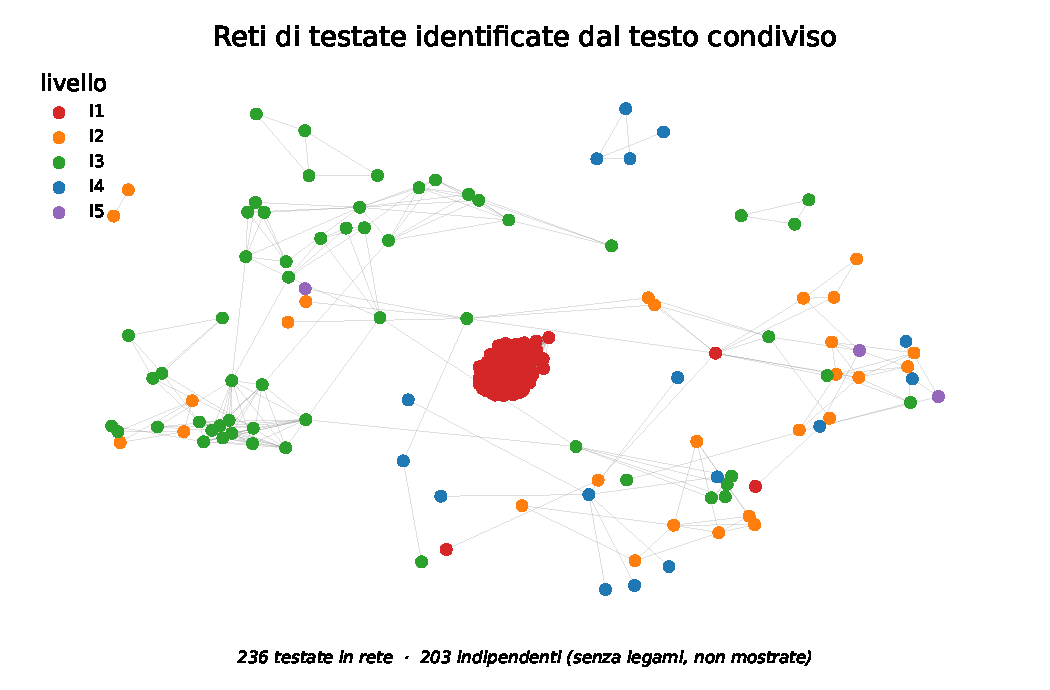
\includegraphics[width=\textwidth]{fig_primo_rete.pdf}\\
      {\scriptsize Un punto = una testata; una linea = almeno 2 articoli quasi uguali. La distanza nel disegno non misura nulla.}
    \end{column}
  \end{columns}
\end{frame}

\begin{frame}{Chi c'\`e dietro una rete: l'owner di NewsGuard}
  \vfill
  \begin{itemize}[<+->]
    \setlength\itemsep{0.7em}
    \item Per ogni sito NewsGuard indica anche il \hl{proprietario} (campo \hl{Owner}): per esempio Metric Media LLC, Boone Newspapers, Salem Media Group
    \item Le reti le ho trovate \hl{solo dal testo}; l'owner l'ho usato \hl{dopo}, per controllarle:
    \item[] \hl{precisione 0,93}: le testate di una stessa rete hanno quasi sempre lo stesso proprietario
    \item[] \hl{recall 0,87}: le testate di uno stesso proprietario finiscono quasi sempre nella stessa rete
    \item La rete da 131 siti: \hl{tutti di Metric Media LLC}, tutti con lo \hl{stesso punteggio} NewsGuard (32): siti di ``notizie locali'' che pubblicano articoli-modello come quello di prima
    \item[] {\small\itshape Quindi: stessa rete = testo quasi uguale (non sempre identico) e, quasi sempre, stesso proprietario.}
  \end{itemize}
  \vfill
\end{frame}

\begin{frame}{Le reti, livello per livello}
  \centering
  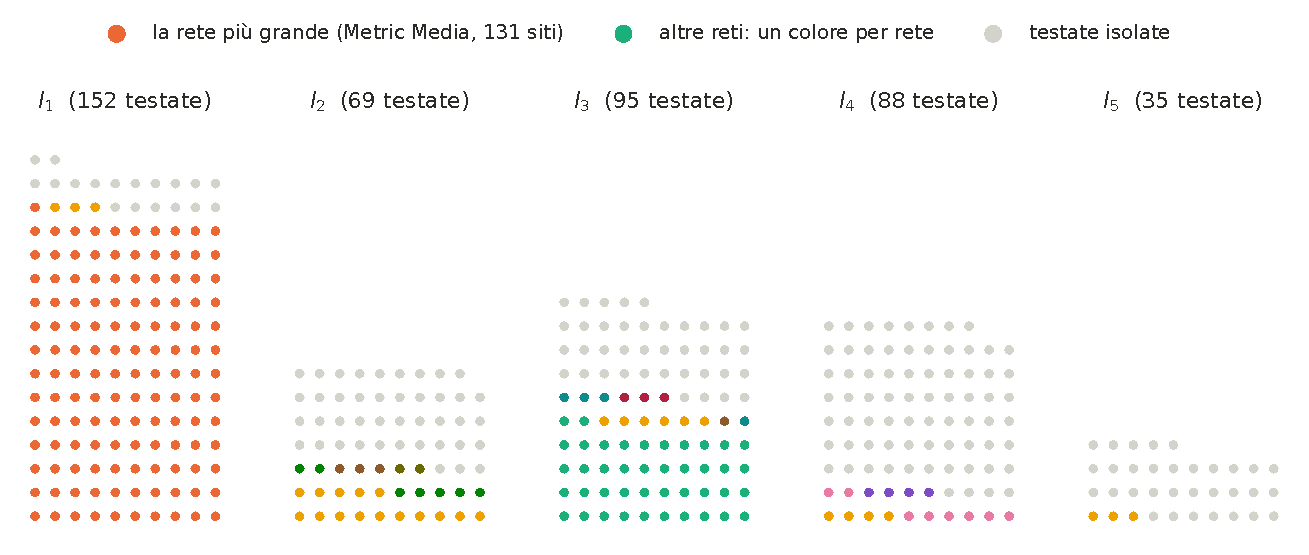
\includegraphics[height=0.56\textheight]{fig_primo_puntini_livelli.pdf}\\[0.1em]
  {\footnotesize Un pallino = una testata; un colore = una rete.}
  \begin{itemize}[<+->]
    \small
    \item $l_1$: \hl{131 testate su 152} sono la stessa rete di Metric Media; solo \hl{20} sono isolate
    \item $l_3$: molte catene di giornali locali; $l_4$ e $l_5$: quasi tutte isolate
  \end{itemize}
\end{frame}

\begin{frame}{Fold per testata: le sorelle stanno da tutte e due le parti}
  \centering
  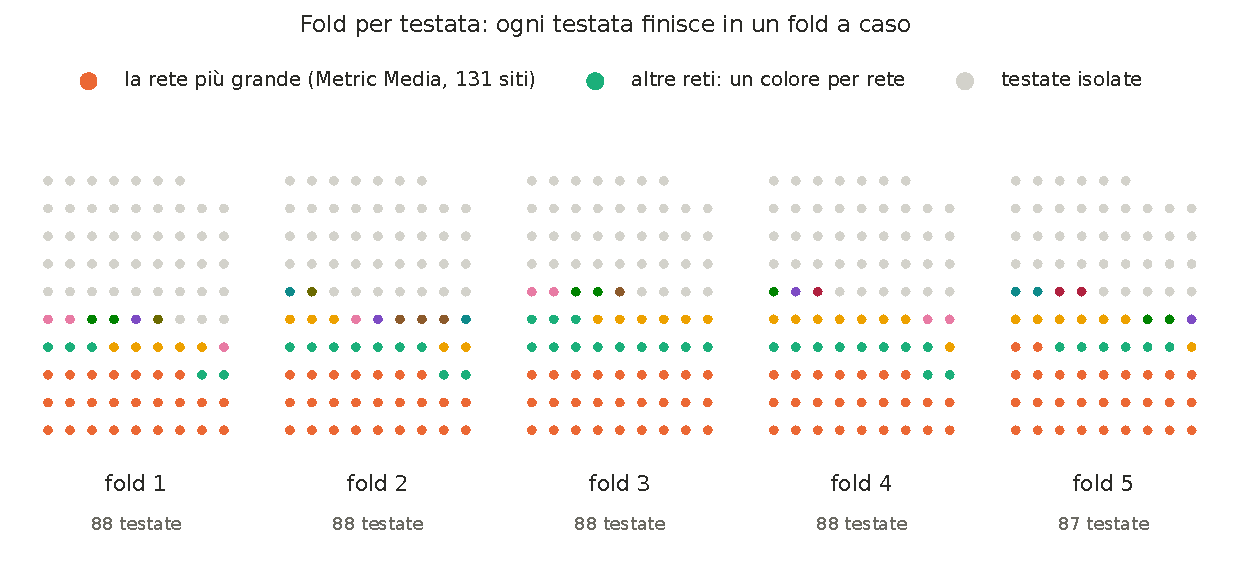
\includegraphics[height=0.56\textheight]{fig_primo_fold_testata.pdf}\\[0.1em]
  \begin{itemize}[<+->]
    \small
    \item Come nel paper: ogni testata va in un fold \hl{a caso}, e i 131 siti di Metric Media si spargono in \hl{tutti e 5} i fold (25--29 per fold)
    \item Lo stesso per le altre reti: ogni colore compare in pi\`u fold, in media \hl{3,5}
    \item Quando il fold 1 \`e il test, gli altri \hl{106 siti} di Metric Media sono nel training: il modello ha gi\`a visto gli stessi articoli-modello
  \end{itemize}
\end{frame}

\begin{frame}{Ripulire il primo dataset: cosa ho tolto e come}
  \vspace{0.2em}
  \centering\footnotesize
  \begin{tabular}{p{0.04\textwidth}p{0.34\textwidth}p{0.25\textwidth}p{0.25\textwidth}}
    \toprule
    & \textbf{Regola} & \textbf{Con quale indice} & \textbf{Quanto} \\
    \midrule
    1 & lo stesso articolo su pi\`u testate: se ne tiene \hl{una copia} & $J \geq 0{,}9$ (stesso testo con poche parole cambiate) & $-$1.835 articoli \\
    2 & copie rimaste tra \hl{reti diverse}: si tolgono tutte e due & $J \geq 0{,}5$ & $-$46 articoli \\
    3 & \hl{paragrafi identici} in almeno 2 testate (didascalie, appelli, avvisi): tolti \hl{dal testo}, l'articolo resta & uguaglianza del paragrafo normalizzato & 5,5\% delle parole \\
    4 & articoli rimasti con \hl{100 parole o meno} & --- & $-$1.325 articoli \\
    \bottomrule
  \end{tabular}\\[0.5em]
  \raggedright
  \begin{itemize}[<+->]
    \item Verifica: coppie di articoli quasi uguali tra reti diverse, rifacendo il MinHash sul testo pulito: da \hl{1,45 milioni} a \hl{0}
    \item Le regole \hl{non guardano le etichette}: si applicano uguali a tutti i livelli
  \end{itemize}
\end{frame}

\begin{frame}{Pulito e valutato per gruppo, il primo dataset non basta}
  \begin{columns}[c]
    \begin{column}{0.56\textwidth}
      \centering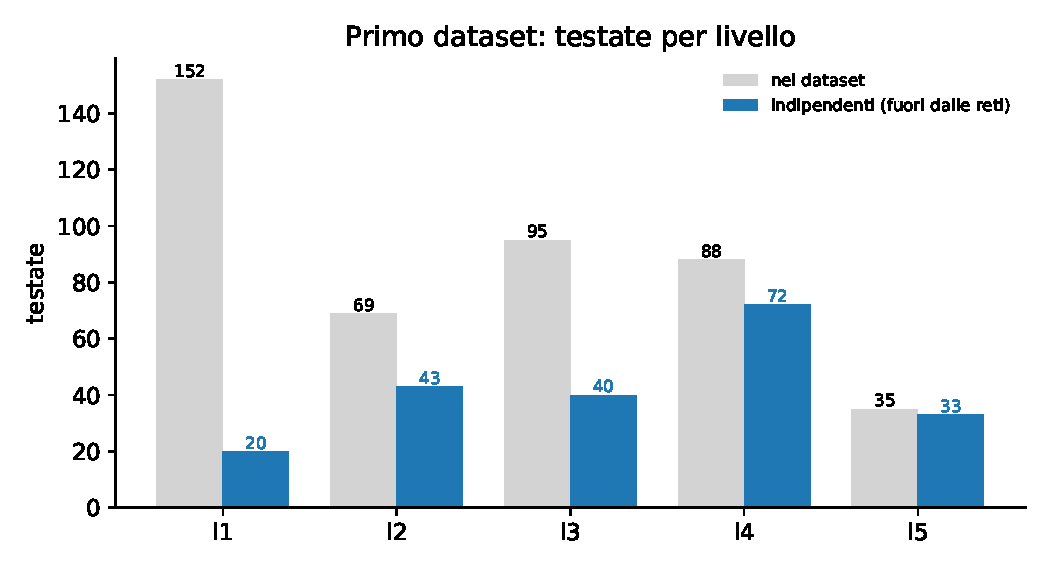
\includegraphics[width=\textwidth]{fig_primo_prima_dopo.pdf}
    \end{column}
    \begin{column}{0.44\textwidth}
      \begin{itemize}[<+->]
        \setlength\itemsep{0.6em}
        \item TF-IDF sul dataset pulito, fold per gruppo: \hl{0,40} di accuratezza, \hl{0,33} di F1 macro
        \item Testate \hl{indipendenti} (fuori dalle reti): solo \hl{20 $l_1$}; il resto di $l_1$ \`e una rete sola, che conta come \hl{un} esempio
        \item Troppo poche testate indipendenti per livello: per andare avanti serve un \hl{dataset nuovo}, pi\`u grande, pulito con lo stesso rigore
      \end{itemize}
    \end{column}
  \end{columns}
\end{frame}

% ===================================================================================================
\divider{Il nuovo dataset}{come l'ho costruito, passo per passo}

\begin{frame}{Lo scraping: due giri nella stessa settimana}
  \begin{itemize}[<+->]
    \setlength\itemsep{0.6em}
    \item \hl{13 ottobre}, primo giro: le testate NewsGuard in inglese, con un punteggio, il cui argomento \`e \hl{esattamente} ``Political news or commentary'': \hl{1.921}
    \item Non bastano: molti siti \hl{bloccano} lo scraper, molti articoli \hl{sporchi} si tolgono, e il tetto di \hl{5 testate per gruppo} (rete o stesso owner, passo 3) ne scarta tante. Serve il dataset \hl{pi\`u grande possibile}
    \item \hl{18 ottobre}, secondo giro, \hl{stesso scraper} e stessi parametri: le testate il cui argomento \hl{contiene} ``Political news or commentary'' insieme ad altri: \hl{+1.207}. Nessuna testata in comune: gli articoli dei due giri si \hl{sommano}
    \item In tutto \hl{3.128} testate tentate, \hl{1.528} raggiunte (bloccata quasi tutta una rete di 1.076 siti $l_1$, pi\`u 176 altre)
    \item In \hl{ordine casuale} e \hl{senza guardare il livello}; fino a 200 articoli recenti per testata, con l'\hl{HTML grezzo}
    \item I due giri sono a \hl{5 giorni} di distanza, con lo stesso strumento: un dataset \hl{coerente}
  \end{itemize}
\end{frame}

\begin{frame}{Prima di questo dataset: altri tentativi}
  \vfill
  \begin{itemize}[<+->]
    \setlength\itemsep{0.9em}
    \item Prima di arrivare qui ho fatto \hl{altri tentativi}, provando \hl{pi\`u strategie di pulizia}
    \item Ogni volta il feature \hl{batteva ancora} i transformer, e in parte per lo \hl{sporco} rimasto nel dataset: testo del sito ripetuto in tutti gli articoli, pagine uguali per tutta una testata, reti di siti non separate
    \item Allora ho reso la pulizia \hl{pi\`u aggressiva}: non pi\`u solo le copie tra testate, come nel primo dataset, ma anche il testo che appartiene al sito e non all'articolo, e le reti trovate anche dall'HTML
    \item Con un limite: si toglie solo quello che \hl{non \`e dell'articolo}; citazioni e pezzi ripresi restano
  \end{itemize}
  \vfill
\end{frame}

\begin{frame}{Come ho costruito il dataset, in breve}
  \vfill
  \begin{enumerate}[<+->]
    \setlength\itemsep{1em}
    \item \hl{Pulire il testo degli articoli}: togliere quello che non \`e dell'articolo ma \hl{del sito} (appelli, firme, titolo ripetuto, data). Un modello lo userebbe per riconoscere il sito, non l'affidabilit\`a
    \item \hl{Trovare le testate parenti} (le reti), \hl{senza guardare NewsGuard}: dalle tracce che lasciano, come testi uguali, stessi codici nell'HTML, stessi autori
    \item \hl{Fare i gruppi e i fold}: le testate parenti vanno tutte dalla stessa parte, e nessun gruppo pu\`o essere troppo grande
  \end{enumerate}
  \vfill
  \visible<4->{\small Ogni passo \`e una \hl{regola scritta nel codice}, applicata uguale a tutte le testate: \hl{nessun testo tolto a mano} o da un LLM. Rieseguendo i notebook (random state fissati) dai dati dello scraping esce sempre lo stesso dataset.}
\end{frame}

\begin{frame}{1. Pulire gli articoli}
  \begin{itemize}[<+->]
    \setlength\itemsep{0.5em}
    \small
    \item Si toglie dal testo quello che \hl{appartiene al sito}, non all'articolo:
    \item[] le frasi che si \hl{ripetono} in molti articoli della stessa testata: appelli, firme, ``iscriviti alla newsletter''. Per esempio truthout.org ha lo stesso appello per le donazioni in \hl{200 articoli su 200}
    \item[] la \hl{cornice della pagina}: il titolo e la data che alcuni siti mettono all'inizio del testo
    \item Si tolgono gli articoli \hl{vecchi} (prima del 2025), i \hl{doppioni} dello stesso pezzo e quelli rimasti \hl{troppo corti}
    \item Sono \hl{impronte del sito}: lasciate l\`i, un modello riconoscerebbe la testata invece di leggere l'articolo
    \item Tutto con \hl{regole automatiche} nel codice, nessuna modifica a mano. Risultato: via il 5\% delle parole; da 101.887 a \hl{76.091} articoli
    \item[] {\small\itshape Con lo stesso MinHash del primo dataset si trovano anche le copie tra testate: servono al passo 2.}
  \end{itemize}
\end{frame}

\begin{frame}{2. Trovare le testate parenti: le tracce}
  \vspace{0.1em}
  \centering\scriptsize
  \begin{tabular}{p{0.15\textwidth}p{0.52\textwidth}p{0.24\textwidth}}
    \toprule
    \textbf{Traccia} & \textbf{Quando due testate sono parenti} & \textbf{Esempio} \\
    \midrule
    copie & hanno articoli quasi uguali in comune (MinHash, $J \geq 0{,}5$): almeno 2, e almeno il 10\% degli articoli della pi\`u piccola & catene di giornali locali \\
    codici\newline di account & nell'HTML di ogni pagina c'\`e il \hl{numero di conto} di AdSense, Google Analytics, pixel di Facebook\dots{} (es.\ \texttt{ca-pub-1234\dots}): due siti con \hl{lo stesso numero} usano lo stesso conto. Conta solo se \`e in almeno met\`a delle pagine & FiveZero: 18 siti, un solo conto AdSense \\
    privacy policy & il link ``Privacy policy'' porta alla \hl{stessa pagina} su un altro dominio, cio\`e lo stesso titolare. Non contano Google, WordPress, Substack e simili, uguali per tutti i clienti & 8 siti, tutti verso la privacy policy di \texttt{salemmedia.com} \\
    dominio & sottodomini dello stesso sito, o la homepage che \hl{reindirizza} allo stesso dominio & le edizioni di HuffPost \\
    autori & la firma dell'articolo: gli \hl{stessi nomi di persona} (non ``Staff'' o le agenzie) firmano almeno il 10\% degli articoli della pi\`u piccola & la rete da 426 siti \\
    \bottomrule
  \end{tabular}\\[0.5em]
  \raggedright\footnotesize
  \begin{itemize}[<+->]
    \item Basta \hl{una} traccia per collegare due testate; una \hl{rete} = testate collegate, anche a catena (come nel primo dataset)
    \item Le soglie del 10\% evitano di collegare due testate per un pezzo d'agenzia o un collaboratore in comune
  \end{itemize}
\end{frame}

\begin{frame}{2. Le reti trovate}
  \begin{columns}[c]
    \begin{column}{0.62\textwidth}
      \centering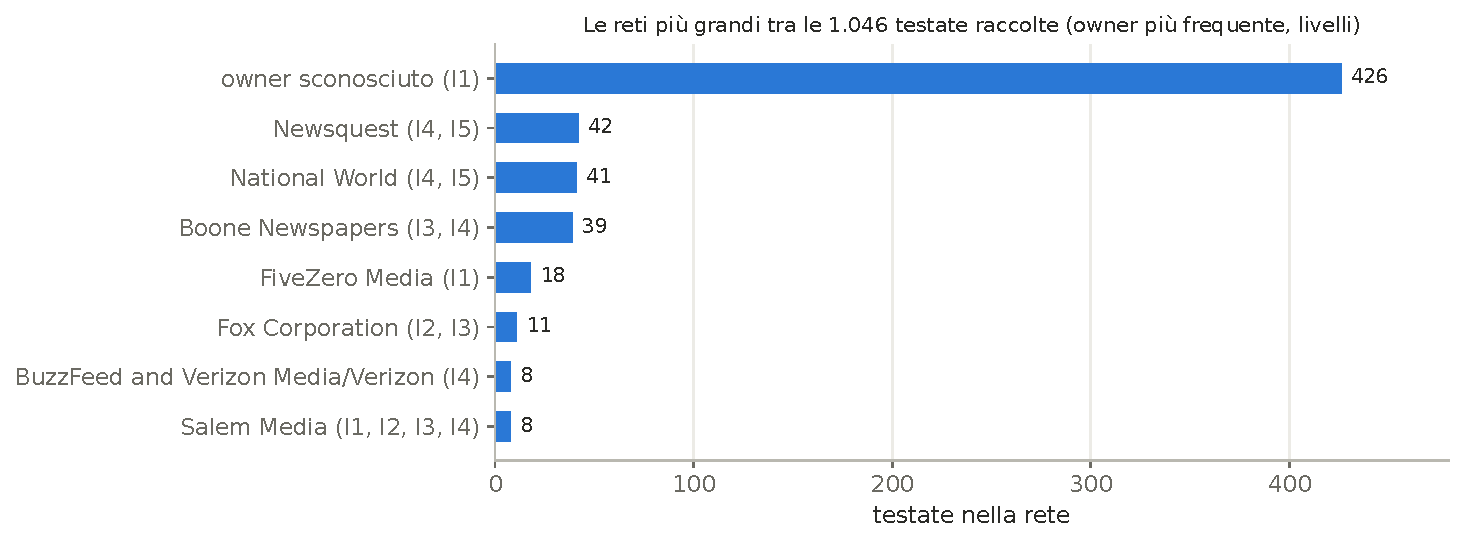
\includegraphics[width=\textwidth]{fig_reti_grandi.pdf}
    \end{column}
    \begin{column}{0.38\textwidth}
      \begin{itemize}[<+->]
        \setlength\itemsep{0.6em}
        \small
        \item \hl{725 testate su 1.046} stanno in una rete con altre
        \item La pi\`u grande ha \hl{426 siti}, legati soprattutto dagli \hl{stessi autori}. Per NewsGuard l'owner \`e \hl{sconosciuto}
        \item Controllo a parte: tutti hanno lo \hl{stesso punteggio} (5) e nel campo ``Parent Domain'' di NewsGuard \hl{425 su 426} dicono \texttt{naturalnews.com}. \`E la rete di Natural News
      \end{itemize}
    \end{column}
  \end{columns}
\end{frame}

\begin{frame}{2. Il controllo con l'owner di NewsGuard}
  \begin{columns}[c]
    \begin{column}{0.54\textwidth}
      \centering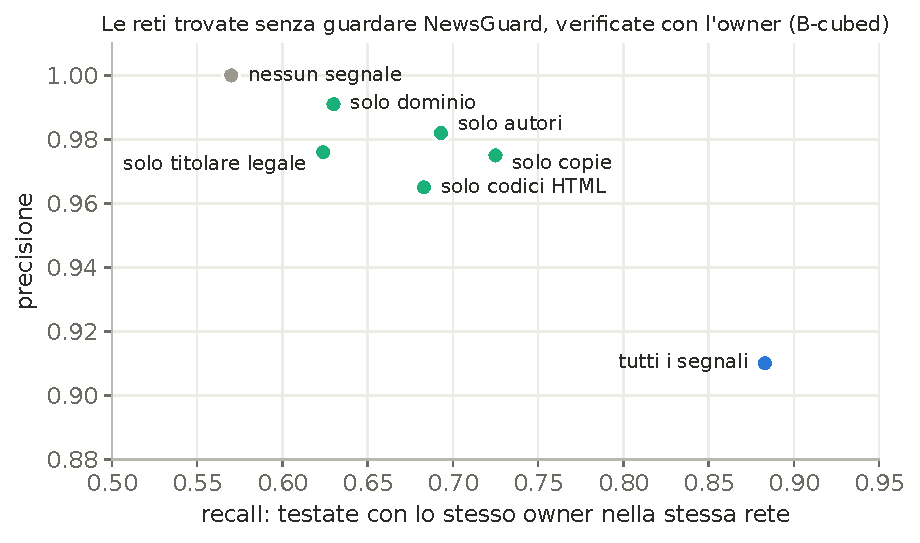
\includegraphics[width=\textwidth]{fig_reti_verifica.pdf}
    \end{column}
    \begin{column}{0.46\textwidth}
      \begin{itemize}[<+->]
        \setlength\itemsep{0.5em}
        \small
        \item Le reti le ho trovate \hl{senza} l'owner: ora lo uso per vedere se sono giuste
        \item Per ogni testata con un owner noto:
        \item[] \hl{precisione}: le testate della sua rete hanno il suo stesso owner?
        \item[] \hl{recall}: le testate del suo owner sono nella sua rete?
        \item[] e poi la media su tutte le testate
        \item Ogni traccia da sola \`e precisa ma trova poco; \hl{tutte insieme}: precisione \hl{0,91}, recall \hl{0,88}
        \item Le testate con owner sconosciuto non entrano nel conto: si controllano a parte, come Natural News
      \end{itemize}
    \end{column}
  \end{columns}
\end{frame}

\begin{frame}{3. I gruppi}
  \vfill
  \begin{itemize}[<+->]
    \setlength\itemsep{1em}
    \item \hl{Gruppo} = rete trovata \hl{oppure} stesso owner NewsGuard: basta uno dei due. L'owner aggiunge le parentele che non lasciano tracce
    \item Lo stesso articolo in \hl{due gruppi diversi}: si tiene la copia pi\`u vecchia ($-$461 articoli). Cos\`i lo stesso testo non sta mai nel training e nel test
    \item Testate con almeno \hl{20 articoli} (per il voto di maggioranza): \hl{702}
  \end{itemize}
  \vfill
\end{frame}

\begin{frame}{3. I gruppi, livello per livello}
  \centering
  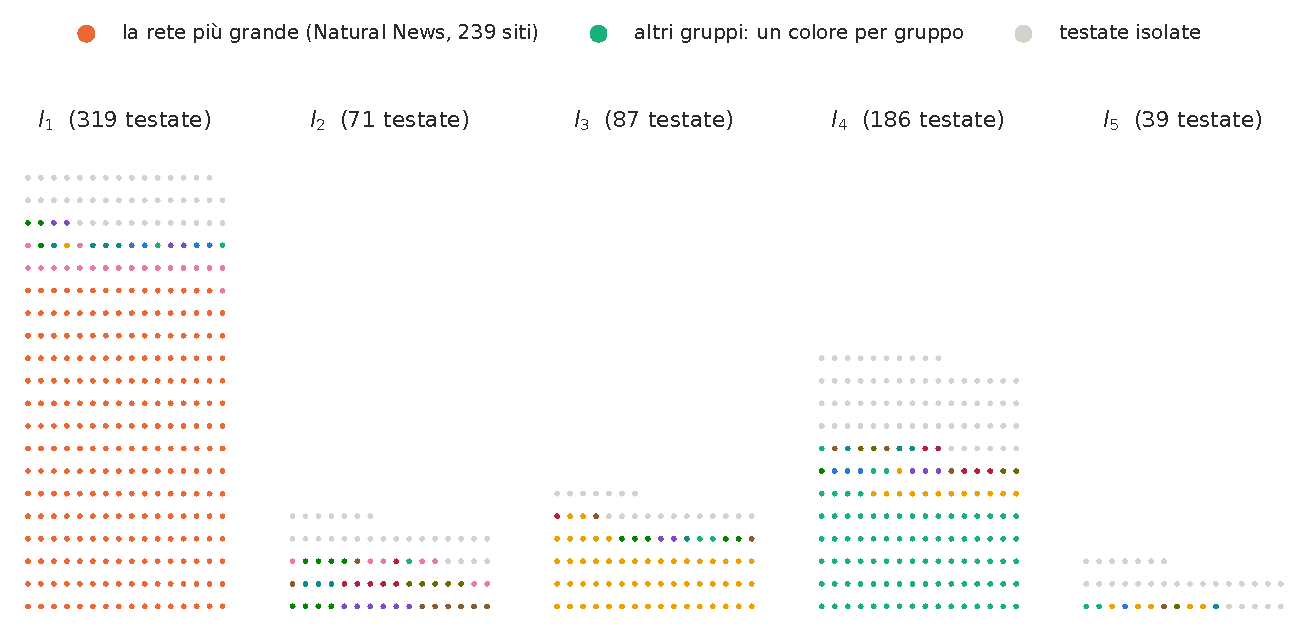
\includegraphics[height=0.6\textheight]{fig_nuovo_prima_tetto.pdf}\\[0.2em]
  {\footnotesize Le 702 testate con almeno 20 articoli. Un pallino = una testata; un colore = un gruppo.}
  \begin{itemize}[<+->]
    \small
    \item Natural News fa \hl{239 delle 319} testate $l_1$: lo stesso problema di Metric Media nel primo dataset
  \end{itemize}
\end{frame}

\begin{frame}{3. Il tetto e i fold}
  \begin{columns}[c]
    \begin{column}{0.5\textwidth}
      \begin{itemize}[<+->]
        \setlength\itemsep{0.7em}
        \item Al massimo \hl{5 testate per gruppo}, scelte \hl{a caso}: Natural News conta come gli altri gruppi, non riempie pi\`u $l_1$
        \item Restano \hl{304 testate} in \hl{220 gruppi}
        \item \hl{5 fold per gruppo}: ogni gruppo sta in un fold solo, e ogni fold ha lo stesso numero di testate per livello
      \end{itemize}
    \end{column}
    \begin{column}{0.5\textwidth}
      \centering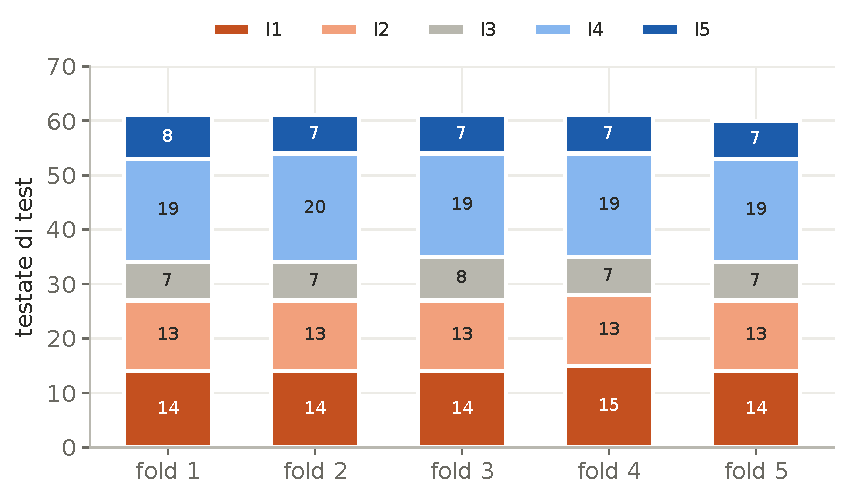
\includegraphics[width=\textwidth]{fig_fold_bilanciati.pdf}\\
      {\footnotesize Testate per livello in ogni fold di test}
    \end{column}
  \end{columns}
\end{frame}

\begin{frame}{Quanto resta a ogni passo}
  \centering
  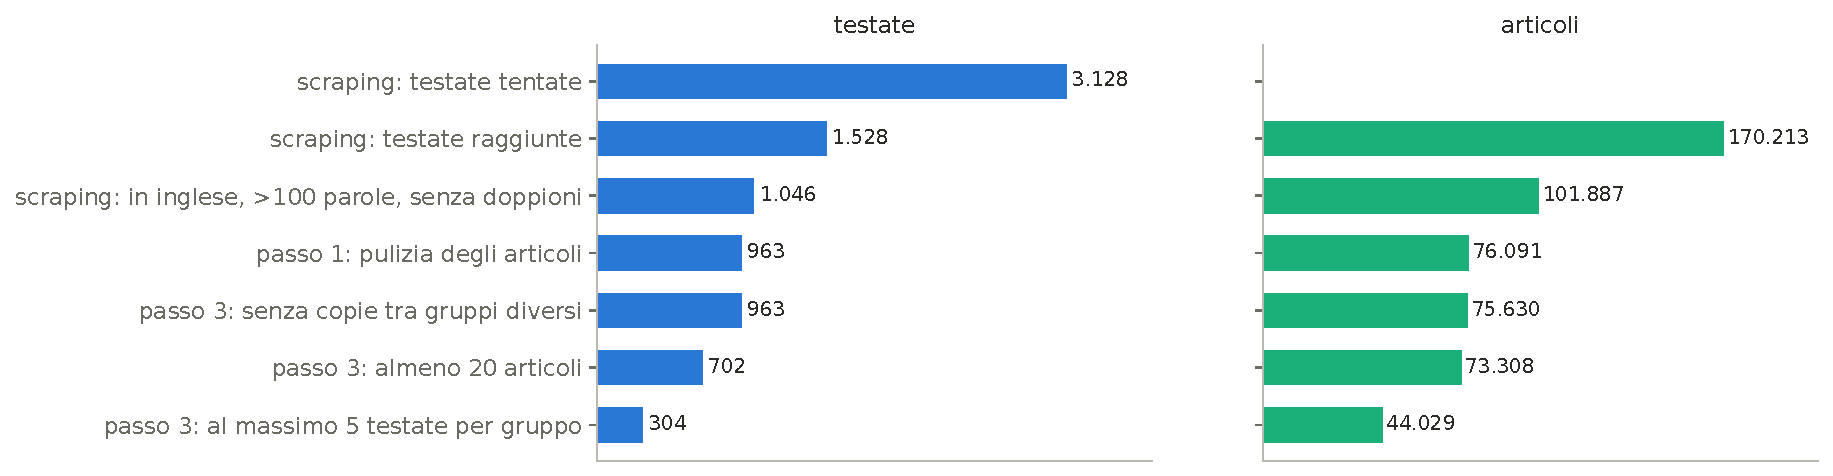
\includegraphics[width=0.96\textwidth]{fig_nuovo_imbuto.pdf}\\[0.4em]
  {\footnotesize Il passo 2 non toglie articoli: serve a fare i gruppi.}
\end{frame}

\begin{frame}{Il dataset finale}
  \centering
  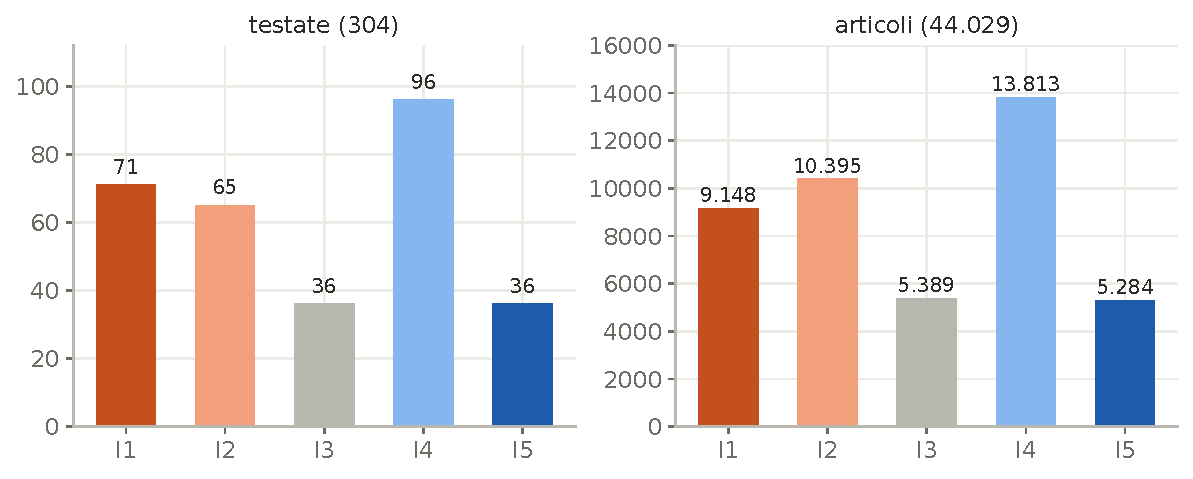
\includegraphics[width=0.85\textwidth]{fig_nuovo_composizione.pdf}\\[0.4em]
  \begin{itemize}[<+->]
    \item \hl{304 testate}, \hl{44.029 articoli}, \hl{220 gruppi} indipendenti
    \item Pi\`u del doppio delle testate $l_1$ indipendenti rispetto al primo dataset (56 gruppi contro 20)
  \end{itemize}
\end{frame}

% ===================================================================================================
\divider{La sporcizia \`e andata?}{gli stessi grafici, sul dataset nuovo}

\begin{frame}{Le reti livello per livello, ora}
  \centering
  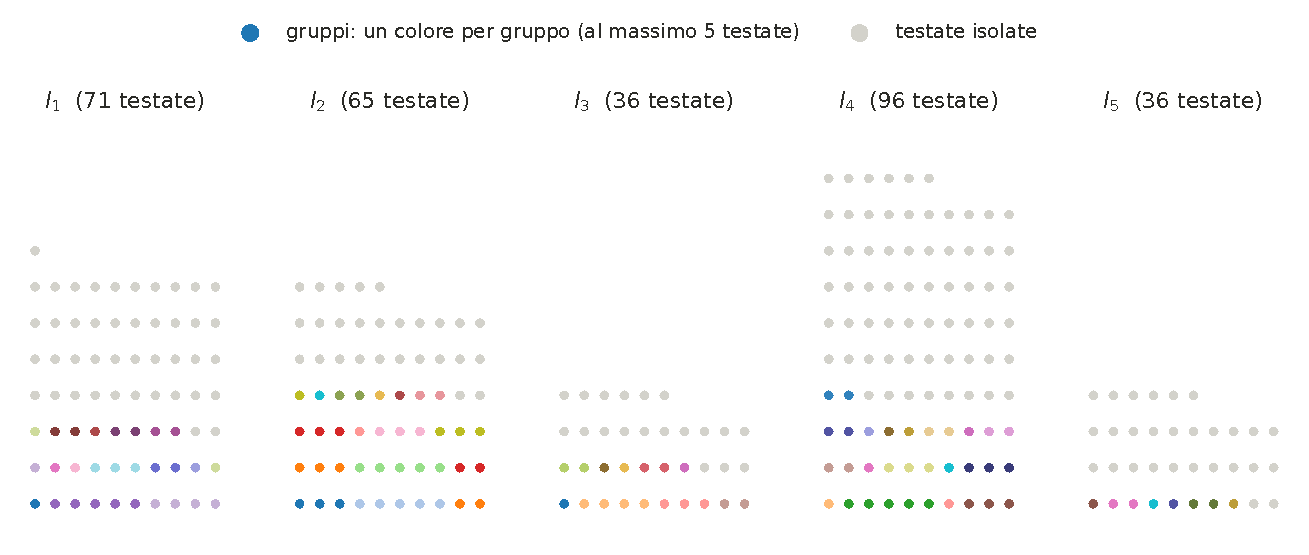
\includegraphics[height=0.56\textheight]{fig_nuovo_puntini_livelli.pdf}\\[0.1em]
  {\footnotesize Un pallino = una testata; un colore = un gruppo.}
  \begin{itemize}[<+->]
    \small
    \item Prima: \hl{131 testate $l_1$ su 152} erano una rete sola. Ora nessun gruppo ha pi\`u di \hl{5 testate}
    \item \hl{181 testate isolate} e \hl{123} in 39 gruppi piccoli; in $l_1$, 43 isolate su 71
  \end{itemize}
\end{frame}

\begin{frame}{I fold, ora}
  \centering
  \only<1>{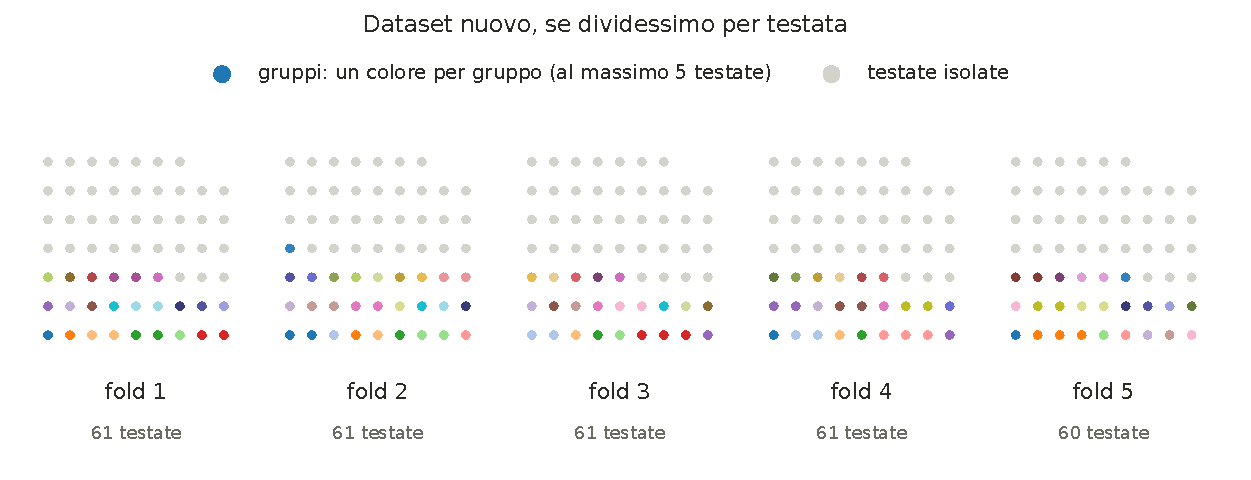
\includegraphics[height=0.5\textheight]{fig_nuovo_fold_testata.pdf}}%
  \only<2->{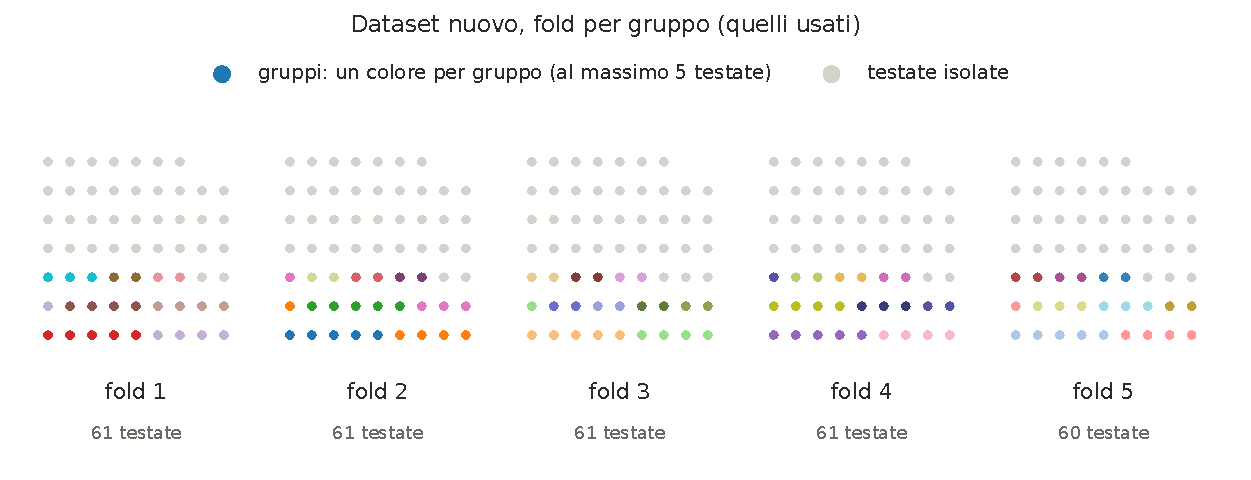
\includegraphics[height=0.5\textheight]{fig_nuovo_fold_gruppo.pdf}}\\[0.1em]
  \begin{itemize}
    \small
    \item<1-> Se dividessimo \hl{per testata}, un gruppo starebbe in media in \hl{2,4 fold}: le sorelle di nuovo da tutte e due le parti
    \item<2-> Con i fold \hl{per gruppo} (quelli usati) ogni colore sta in \hl{un solo fold}
    \item<3-> \`E una divisione \hl{in pi\`u}, non al posto di quella per testata: gli articoli di una testata stanno \hl{sempre} in un solo fold, e in pi\`u le testate di un gruppo stanno insieme
  \end{itemize}
\end{frame}

% ===================================================================================================
\divider{Risultati}{TF-IDF contro transformer, sul dataset nuovo}

\begin{frame}{Come sono arrivato alla ricetta dei transformer}
    \centering\scriptsize
  \begin{tabular}{p{0.56\textwidth}p{0.36\textwidth}}
    \toprule
    \textbf{Cosa \`e successo nei tentativi precedenti} & \textbf{Cosa ho cambiato} \\
    \midrule
    Con le pagine del sito ModernBERT \hl{imparava a memoria} le testate: le pagine erano uguali in tutti i loro articoli, e la loss di training andava a zero gi\`a nella prima epoca & solo il testo degli articoli, pulito \\
    \addlinespace
    Le testate con tanti articoli pesavano di pi\`u nell'addestramento, e i livelli con poche testate rischiavano di essere ignorati; l'analisi diceva che 5--20 articoli per testata bastano quasi del tutto & \hl{20 articoli a caso per testata} a ogni epoca; \hl{pesi di classe} \\
    \addlinespace
    L'early stopping sceglieva l'epoca su una validazione di circa 22 testate: la F1 saltava da un'epoca all'altra (0,17 $\to$ 0,37 $\to$ 0,42 $\to$ 0,39) e la scelta era quasi a caso. E dopo 1--2 epoche il modello cominciava a imparare a memoria & \hl{2 epoche fisse}, niente early stopping \\
    \addlinespace
    2048 token non andavano meglio di 1024 (F1 0,242 contro 0,255) & \hl{1024 token} \\
    \addlinespace
    Cambiando solo il seed, la F1 cambiava quanto tra un modello e l'altro & \hl{3 seed} e la loro media \\
    \addlinespace
    Un ModernBERT \hl{congelato}, senza addestramento, andava quasi come quello addestrato & provare gli \hl{embedding congelati} \\
    \addlinespace
    Large e base erano pari, ma su 193 testate & riprovare il \hl{large} sul dataset pi\`u grande \\
    \bottomrule
  \end{tabular}
\end{frame}

\begin{frame}{La ricetta finale dei transformer}
  \begin{itemize}[<+->]
    \setlength\itemsep{0.7em}
    \item \hl{Fine-tuning}: si prende ModernBERT gi\`a pre-addestrato e lo si addestra ancora, sul nostro compito: leggere \hl{un articolo} e dire il livello della sua testata
    \item Per giudicare una \hl{testata} si fa la \hl{media delle probabilit\`a} di tutti i suoi articoli
    \item Due taglie, \hl{base} (150 milioni di parametri) e \hl{large} (400 milioni), per vedere se un modello pi\`u grande aiuta
    \item La stessa ricetta per tutti, quella della slide prima: primi \hl{1024 token} di ogni articolo, \hl{2 epoche}, a ogni epoca \hl{20 articoli a caso per testata}, \hl{pesi di classe}
    \item Il TF-IDF in due versioni: con i parametri scelti in una validazione sul solo training (\hl{riferimento}, fissato prima) e con quelli di default
  \end{itemize}
\end{frame}

\begin{frame}{Seed, ensemble ed embedding congelati}
  \begin{itemize}[<+->]
    \setlength\itemsep{0.6em}
    \item Il \hl{seed} \`e il numero che fissa il caso nell'addestramento: da dove parte il modello, quali 20 articoli si pescano, in che ordine. Con lo stesso dataset e la stessa ricetta, seed diversi danno modelli diversi
    \item Quanto diversi? Qui ModernBERT-base fa F1 da \hl{0,33 a 0,38} a seconda del seed: tanto quanto la differenza tra due modelli
    \item Per questo ogni ModernBERT gira con \hl{3 seed} (42, 1, 2), e il risultato principale \`e l'\hl{ensemble}: la media delle probabilit\`a dei tre modelli, che dipende meno dal caso. Il ``seed 42'' da solo lo riporto solo per far vedere quanto varia, non si sceglie il migliore
    \item \hl{Embedding congelati} (e5-large, bge-large): il modello \hl{non si addestra}. Trasforma ogni articolo in 1024 numeri, si fa la media per testata e sopra si mette la stessa regressione logistica del TF-IDF
    \item[] Costano poco e \hl{non possono imparare a memoria} le testate: dicono se basta una rappresentazione generica del testo
  \end{itemize}
\end{frame}

\begin{frame}{I risultati}
  \vspace{0.2em}
  \centering\footnotesize
  \resizebox{\textwidth}{!}{%
  \begin{tabular}{lcccccc}
    \toprule
    \textbf{Modello} & \textbf{F1 macro} & \textbf{acc.\ 5 cl.} & \textbf{tol.\ 0,5} & \textbf{tol.\ 1} & \textbf{binario} & \textbf{F1 bin.} \\
    \midrule
    \textbf{TF-IDF, parametri in validazione} (riferimento) & 0,380 & 0,424 & 0,597 & 0,770 & 0,740 & 0,740 \\
    TF-IDF, parametri di default & 0,368 & \textbf{0,454} & \textbf{0,628} & \textbf{0,803} & \textbf{0,776} & \textbf{0,776} \\
    \midrule
    ModernBERT-base, 3 seed & 0,366 & 0,398 & 0,589 & 0,780 & 0,717 & 0,717 \\
    ModernBERT-large, 3 seed & 0,348 & 0,405 & 0,602 & 0,799 & 0,743 & 0,742 \\
    ModernBERT-base, seed 42 & \textbf{0,383} & 0,424 & 0,599 & 0,773 & 0,720 & 0,720 \\
    \midrule
    e5-large congelato & 0,331 & 0,391 & 0,589 & 0,786 & 0,727 & 0,723 \\
    bge-large congelato & 0,325 & 0,382 & 0,586 & 0,789 & 0,730 & 0,729 \\
    \midrule
    classe di maggioranza & 0,096 & 0,316 & 0,434 & 0,553 & 0,553 & 0,356 \\
    a caso & 0,214 & 0,243 & 0,388 & 0,533 & 0,510 & 0,505 \\
    \bottomrule
  \end{tabular}}\\[0.4em]
  \raggedright{\scriptsize\itshape Per testata, 304 testate, fold per gruppo. Tolerant: un errore di un livello vale mezzo punto (0,5) o un punto (1).}
\end{frame}

\begin{frame}{Con gli intervalli}
  \centering
  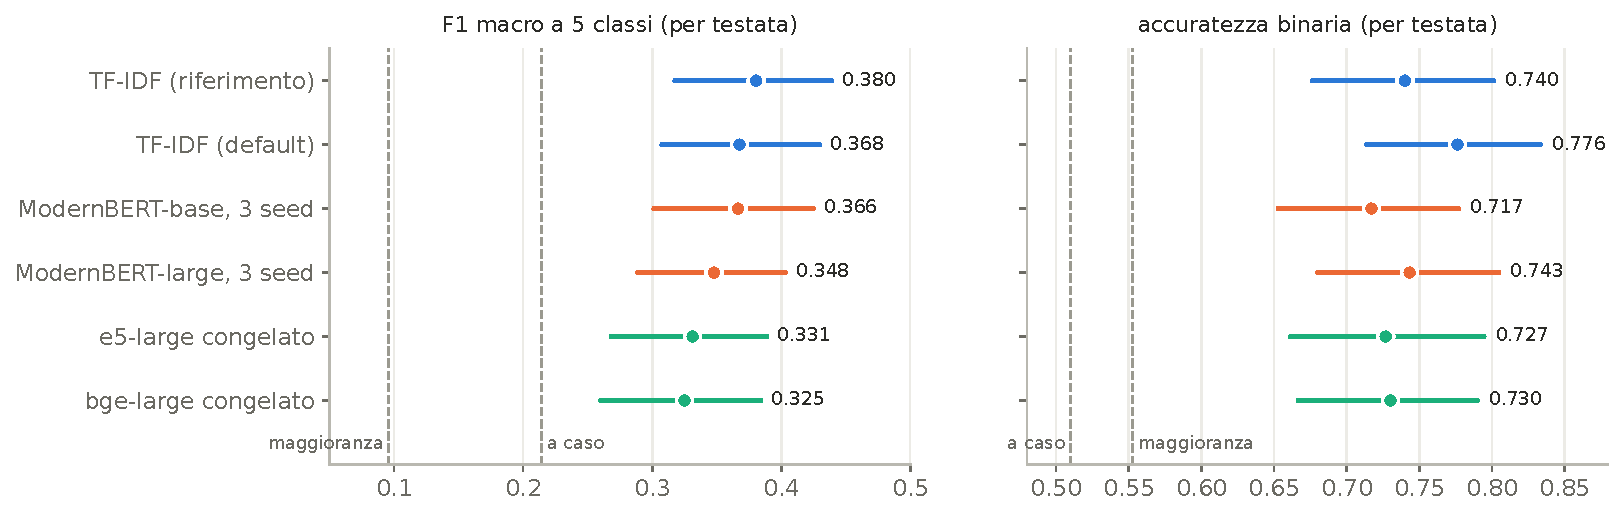
\includegraphics[width=\textwidth]{fig_risultati_intervalli.pdf}\\[0.2em]
  \begin{itemize}[<+->]
    \footnotesize
    \item Tutti i modelli stanno \hl{ben sopra} maggioranza e caso: dal solo testo un segnale c'\`e
    \item \hl{Nessun transformer batte il feature} in modo significativo: le differenze stanno tutte negli intervalli
    \item Il modello pi\`u grande e gli embedding congelati \hl{non aiutano}
  \end{itemize}
\end{frame}

\begin{frame}{Chi riconosce cosa}
  \begin{columns}[c]
    \begin{column}{0.6\textwidth}
      \centering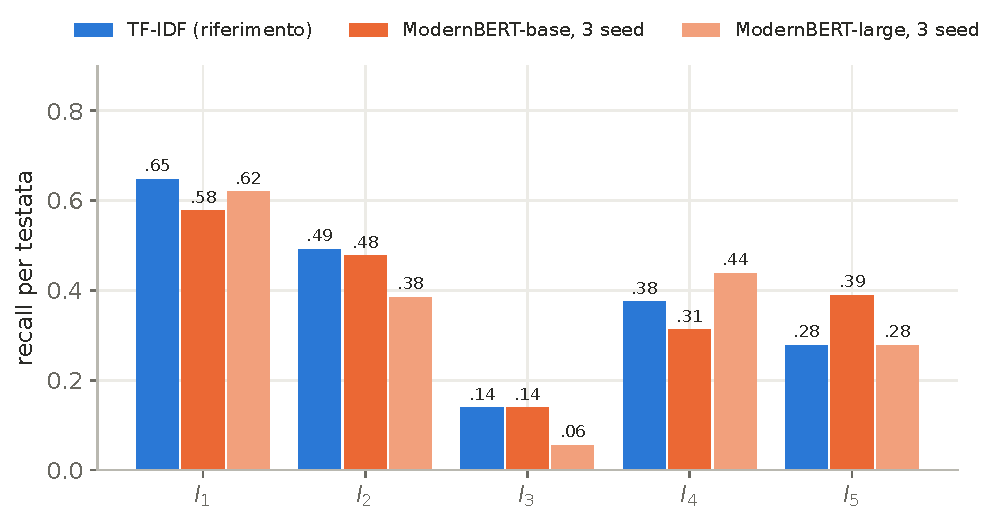
\includegraphics[width=\textwidth]{fig_recall_livelli.pdf}
    \end{column}
    \begin{column}{0.4\textwidth}
      \begin{itemize}[<+->]
        \setlength\itemsep{0.6em}
        \item Il feature riconosce meglio le testate \hl{inaffidabili} ($l_1$)
        \item ModernBERT-base riconosce meglio le \hl{pi\`u affidabili} ($l_5$); il large le $l_4$
        \item Gli errori sono \hl{diversi}: i due modelli sono complementari
      \end{itemize}
    \end{column}
  \end{columns}
\end{frame}

\begin{frame}{E senza la classe $l_1$?}
  \vspace{0.1em}
  \centering\footnotesize
  \resizebox{\textwidth}{!}{%
  \begin{tabular}{lcccccc}
    \toprule
    \textbf{Modello} & \textbf{F1 macro} & \textbf{acc.\ 4 cl.} & \textbf{tol.\ 0,5} & \textbf{tol.\ 1} & \textbf{binario} & \textbf{F1 bin.} \\
    \midrule
    \textbf{TF-IDF, parametri in validazione} (riferimento) & 0,358 & 0,408 & 0,586 & 0,764 & 0,712 & 0,667 \\
    TF-IDF, parametri di default & 0,364 & \textbf{0,451} & 0,616 & 0,781 & \textbf{0,734} & 0,683 \\
    \midrule
    ModernBERT-base, 3 seed & 0,355 & 0,395 & 0,607 & 0,820 & 0,717 & 0,673 \\
    ModernBERT-large, 3 seed & 0,311 & 0,369 & 0,590 & 0,811 & 0,704 & 0,637 \\
    ModernBERT-base, seed 42 & \textbf{0,379} & 0,433 & \textbf{0,624} & 0,815 & 0,721 & \textbf{0,688} \\
    \midrule
    e5-large congelato & 0,304 & 0,361 & 0,597 & \textbf{0,833} & 0,717 & 0,634 \\
    bge-large congelato & 0,297 & 0,352 & 0,579 & 0,807 & 0,700 & 0,627 \\
    \midrule
    classe di maggioranza ($l_4$) & 0,146 & 0,412 & 0,567 & 0,721 & 0,721 & 0,419 \\
    a caso & 0,251 & 0,300 & 0,479 & 0,657 & 0,584 & 0,485 \\
    \bottomrule
  \end{tabular}}\\[0.4em]
  \raggedright{\scriptsize\itshape 233 testate ($l_2$--$l_5$); i modelli scelgono tra $l_2$ e $l_5$ (le probabilit\`a salvate, senza riaddestrare). Binario: $l_2$ contro $l_3$--$l_5$.}
  \begin{itemize}[<+->]
    \footnotesize
    \item Senza $l_1$ il vantaggio del feature \hl{sparisce}: ModernBERT-base, 3 seed, \`e \hl{pari} (differenza di F1 0,000 [$-$0,07; $+$0,07]) e sulla tolerant 1 meglio
    \item {\itshape Analisi esplorativa, decisa dopo aver visto i risultati}
  \end{itemize}
\end{frame}

\begin{frame}{Perch\'e il feature vince su $l_1$}
  \vspace{0.2em}
  Le parole che spingono di pi\`u verso $l_1$ nel modello TF-IDF sono di due tipi:\\[0.5em]
  \begin{columns}[t]
    \begin{column}{0.5\textwidth}
      \begin{block}{\footnotesize Contenuto e ideologia}
        \footnotesize \textit{president trump, abortion, kiev, lifesitenews, epoch times, preborn}, nomi di stati e regioni\\[0.3em]
        $\to$ segnale vero, ma intrecciato con \hl{temi e orientamento}: un confondente da discutere
      \end{block}
    \end{column}
    \begin{column}{0.5\textwidth}
      \begin{alertblock}{\footnotesize Residui dell'estrazione}
        \footnotesize \textit{pic twitter, https, www, com, youtube, utc}, qualche firma rimasta nel testo\\[0.3em]
        $\to$ resti di tweet, video e link incorporati: i siti $l_1$ ne usano molti di pi\`u, e il TF-IDF li \hl{conta}
      \end{alertblock}
    \end{column}
  \end{columns}
  \vspace{0.6em}
  \begin{itemize}[<+->]
    \item Il vantaggio \hl{non viene dalle reti}: il feature indovina le $l_1$ isolate (30/43) e quelle in un gruppo (20/28) allo stesso modo
    \item I residui di link e contenuti incorporati sono \hl{cornice della pagina}, come titolo e timbro che abbiamo gi\`a tolto
  \end{itemize}
\end{frame}

\begin{frame}{Perch\'e \`e un risultato valido per il paper}
  \vfill
  \begin{itemize}[<+->]
    \setlength\itemsep{0.7em}
    \item \hl{Il problema}: con le testate divise come al solito i numeri sono gonfiati dalle reti (primo dataset: 0,68 $\to$ 0,39)
    \item \hl{Il metodo}: reti trovate senza NewsGuard, da testo e HTML (precisione 0,91, recall 0,88), e valutazione per gruppo; processo deterministico e replicabile
    \item \hl{Il risultato}: con una valutazione onesta il testo da solo d\`a un segnale \hl{moderato} (F1 0,38, binario 0,74--0,78); i transformer \hl{non battono} un modello lessicale ben fatto, ma sbagliano in modo \hl{diverso}
    \item \hl{Il dubbio}: parte del vantaggio del feature su $l_1$ sono residui di link e tweet incorporati
  \end{itemize}
  \vfill
\end{frame}

% ===================================================================================================
\divider{Versione 2}{pi\`u pulizia e pi\`u testate nel training (19--20 ottobre)}

\begin{frame}{Versione 2: cosa ho cambiato}
  \begin{itemize}[<+->]
    \setlength\itemsep{0.6em}
    \item Tutto \hl{deciso prima} di vedere i risultati, stesso scraping, stesse regole di prima pi\`u tre cose:
    \item[] \hl{1. Una regola di pulizia in pi\`u}: via i resti dei contenuti incorporati (link, \texttt{pic.twitter.com}, firme dei tweet, ``View this post on Instagram''). Espressioni regolari fisse, nessun LLM; il testo dei tweet citati resta
    \item[] \hl{2. Pi\`u testate nel training}: il test resta \hl{identico} (le stesse 304 testate, gli stessi fold); nel training entrano anche le altre testate dei gruppi, \hl{863} invece di 304. Un gruppo non pesa mai pi\`u di 5 testate (pesi per TF-IDF ed embedding; per i transformer 5 testate a caso per gruppo, diverse a ogni epoca)
    \item[] \hl{3. Una combinazione fissata a priori}: media 0,5/0,5 delle probabilit\`a di TF-IDF e ModernBERT-base
    \item Due \hl{controlli}: TF-IDF e ModernBERT addestrati solo sulle 304 testate, per misurare l'effetto del training pi\`u grande
  \end{itemize}
\end{frame}

\begin{frame}{Versione 2: la pulizia nuova}
  \vfill
  \begin{itemize}[<+->]
    \setlength\itemsep{0.8em}
    \item Tolti circa \hl{20.000 link} e \hl{16.000 firme} o scritte di contenuti incorporati: lo 0,3\% delle parole
    \item Tocca il \hl{24\%} degli articoli $l_1$ e solo il \hl{3\%} degli $l_5$: era proprio il residuo che il TF-IDF usava per $l_1$
    \item Il test non cambia: \hl{le stesse 304 testate}, 44.012 articoli (17 in meno), gli stessi fold
    \item Ogni passo resta una regola nel codice; pulizia ed esperimenti sono girati da soli sul server, in una notte
  \end{itemize}
  \vfill
\end{frame}

\begin{frame}{Versione 2: i risultati}
  \vspace{0.2em}
  \centering\footnotesize
  \resizebox{\textwidth}{!}{%
  \begin{tabular}{lcccc}
    \toprule
    & \multicolumn{2}{c}{\textbf{F1 macro}} & \multicolumn{2}{c}{\textbf{binario}} \\
    \cmidrule(lr){2-3}\cmidrule(lr){4-5}
    \textbf{Modello} & \textbf{v2} & v1 & \textbf{v2} & v1 \\
    \midrule
    \textbf{TF-IDF, parametri in validazione} (riferimento) & 0,370 & 0,380 & \textbf{0,773} & 0,740 \\
    TF-IDF, parametri di default & \textbf{0,389} & 0,368 & 0,770 & 0,776 \\
    TF-IDF, training solo sulle 304 testate (controllo) & 0,388 & --- & 0,770 & --- \\
    \midrule
    ModernBERT-base, 3 seed & 0,341 & 0,366 & 0,707 & 0,717 \\
    ModernBERT-base, i singoli seed & 0,32 / 0,36 / 0,36 & 0,35 / 0,33 / 0,38 & & \\
    ModernBERT-base s42, training solo sulle 304 (controllo) & 0,341 & --- & 0,694 & --- \\
    \midrule
    e5-large congelato & 0,322 & 0,331 & 0,724 & 0,727 \\
    bge-large congelato & 0,347 & 0,325 & 0,707 & 0,730 \\
    \midrule
    combinazione TF-IDF + ModernBERT (0,5/0,5) & 0,355 & --- & 0,753 & --- \\
    \midrule
    classe di maggioranza & 0,096 & 0,096 & 0,553 & 0,553 \\
    \bottomrule
  \end{tabular}}\\[0.4em]
  \raggedright{\scriptsize\itshape Per testata, le stesse 304 testate, fold per gruppo. ModernBERT-large non \`e girato: la GPU condivisa aveva solo 7 GB liberi, e il large non ci sta.}
\end{frame}

\begin{frame}{Versione 2: cosa ci dice}
  \vfill
  \begin{enumerate}[<+->]
    \setlength\itemsep{0.7em}
    \item La pulizia nuova \hl{non ha messo in difficolt\`a} il TF-IDF (0,37--0,39): i resti di link e tweet non erano il motivo per cui vinceva
    \item Pi\`u testate nel training \hl{non aiutano} in modo chiaro: per il TF-IDF niente, per ModernBERT +0,02 su un solo seed, mentre l'ensemble scende
    \item La combinazione \hl{non batte} il TF-IDF (0,355 contro 0,370)
    \item Tra un seed e l'altro ModernBERT varia di \hl{4 punti}: quanto tutti gli effetti che cerchiamo. Nessuna differenza con il TF-IDF \`e significativa
  \end{enumerate}
  \vspace{0.6em}
  \visible<5->{\small\itshape Due esperimenti fatti bene, lo stesso risultato: sul solo testo, valutato senza le reti, transformer e TF-IDF sono alla pari, con il TF-IDF un po' avanti.}
  \vfill
\end{frame}

% ===================================================================================================
\divider{Perch\'e il TF-IDF va cos\`i bene}{l'analisi del 20 ottobre (Versione 2, \texttt{05\_analisi\_feature})}

\begin{frame}{Il segnale \`e sparso: regge a quasi tutto}
  \begin{columns}[c]
    \begin{column}{0.52\textwidth}
      \centering\small
      \begin{tabular}{lcc}
        \toprule
        \textbf{Il TF-IDF su\dots} & \textbf{F1} & \textbf{binario} \\
        \midrule
        il testo intero & 0,387 & 0,776 \\
        senza nomi propri & 0,383 & 0,760 \\
        senza le 1000 parole pi\`u forti & 0,377 & 0,753 \\
        senza parole funzione & 0,370 & 0,753 \\
        \textbf{solo parole funzione} & \textbf{0,364} & 0,717 \\
        solo le prime 100 parole & 0,344 & 0,730 \\
        \bottomrule
      \end{tabular}\\[0.3em]
      {\scriptsize Stesse 304 testate, fold per gruppo; ogni riga riaddestrata.}
    \end{column}
    \begin{column}{0.48\textwidth}
      \begin{itemize}[<+->]
        \setlength\itemsep{0.6em}
        \small
        \item Non sono i nomi, n\'e poche parole memorizzate
        \item Con \hl{solo le parole funzione} (the, of, which\dots), cio\`e lo stile senza contenuto, si arriva a 0,364
        \item C'\`e in ogni articolo: con \hl{1 articolo} per testata 0,325, con 5 gi\`a 0,372, con 20 il massimo
      \end{itemize}
    \end{column}
  \end{columns}
\end{frame}

\begin{frame}{I livelli sono generi diversi di testata}
  \vspace{0.2em}
  \centering\footnotesize
  \begin{tabular}{lccccc}
    \toprule
    \textbf{Metadati NewsGuard} (quota di testate) & $l_1$ & $l_2$ & $l_3$ & $l_4$ & $l_5$ \\
    \midrule
    orientamento Far Right & 0,69 & 0,32 & 0,25 & 0,05 & 0,00 \\
    argomento ``Conspiracy theories'' & 0,56 & 0,08 & 0,11 & 0,01 & 0,00 \\
    opinione o advocacy & 0,90 & 0,89 & 0,75 & 0,53 & 0,33 \\
    testate fuori dagli Stati Uniti & 0,08 & 0,06 & 0,17 & 0,35 & 0,28 \\
    \bottomrule
  \end{tabular}\\[0.5em]
  \raggedright
  \begin{itemize}[<+->]
    \footnotesize
    \item $l_1$: estrema destra e complotti, siti che riprendono contenuti; \textit{president trump, abortion, media, kiev}; citano le fonti per dominio (\textit{youtube.com, foxnews.com})
    \item $l_2$: notizie conservatrici di parte; \textit{according to, said, fox news, breitbart}
    \item $l_3$: giornali locali; parole forti = nomi di contee e citt\`a, firme di una testata sola: indovina l'11\%
    \item $l_4$ e $l_5$: testate internazionali e d'inchiesta; \textit{per cent, defence, kyiv, Ireland, ProPublica}
  \end{itemize}
\end{frame}

\begin{frame}{L'orientamento politico}
  \begin{itemize}[<+->]
    \setlength\itemsep{0.55em}
    \small
    \item Il TF-IDF \hl{riconosce l'orientamento} dal testo: accuratezza 0,58, contro 0,38 della classe pi\`u frequente
    \item Dentro un orientamento quasi \hl{non batte} il livello pi\`u comune di quell'orientamento: Far Right 0,55 contro 0,58, Slightly Left 0,36 contro 0,52
    \item Senza nessuna parola, i soli \hl{metadati NewsGuard} (orientamento, opinione, argomenti, paese) fanno F1 \hl{0,339}; dodici misure di stile 0,296; le date 0,150 (niente)
    \item[] {\small\itshape Il TF-IDF va bene perch\'e il livello va di pari passo con il genere della testata, che si legge ovunque nel testo. \`E il confondente da scrivere nel paper.}
    \item Ma un segnale \hl{oltre il genere} c'\`e: affidabile s\`i/no \hl{dentro} ogni orientamento, il TF-IDF fa 0,66 di accuratezza bilanciata (il caso fa 0,50); ModernBERT-base 0,54 {\footnotesize (a posteriori, su modelli non addestrati per questo)}
  \end{itemize}
\end{frame}

% ===================================================================================================
\divider{Versione 3: a parit\`a di genere}{il testo distingue l'affidabilit\`a dentro lo stesso orientamento? (lanciata il 20 ottobre)}

\begin{frame}{Versione 3: il disegno, fissato prima dei risultati}
  \begin{itemize}[<+->]
    \setlength\itemsep{0.6em}
    \item Lo \hl{stesso dataset} della Versione 2: stessa pulizia, stesse 304 testate di test, stessi fold per gruppo
    \item Compito \hl{binario}: affidabile = punteggio $\geq 60$
    \item \hl{Pesi a parit\`a di genere}: dentro ogni orientamento NewsGuard (Far Right, Slightly Right, Slightly Left, Far Left, nessuno) affidabili e inaffidabili pesano uguale nel training. Sapere l'orientamento non serve pi\`u
    \item Metrica: \hl{accuratezza bilanciata dentro ogni orientamento}, poi la media. I soli metadati fanno \hl{0,50} per costruzione: tutto quello che sta sopra viene dal testo
    \item TF-IDF (C = 1 e C in validazione interna) e ModernBERT-base con 3 seed e il loro ensemble; nei log, fold per fold, i due modelli sugli stessi fold
    \item[] {\small\itshape Il limite: l'unico orientamento bilanciato \`e Slightly Right (40 testate affidabili, 38 no); Far Right 14 contro 70. Intervalli larghi.}
  \end{itemize}
\end{frame}

\begin{frame}{Versione 3: i risultati}
  \vspace{0.1em}
  \centering\footnotesize
  \resizebox{\textwidth}{!}{%
  \begin{tabular}{lccccccc}
    \toprule
    & \textbf{media sugli} & \textbf{IC 95\%} & \textbf{AUC} & \textbf{Slightly} & \textbf{Far} & \textbf{Slightly} & \textbf{nessun} \\
    \textbf{Modello} & \textbf{orientamenti} & & \textbf{media} & \textbf{Right} & \textbf{Right} & \textbf{Left} & \textbf{orient.} \\
    \midrule
    \textbf{TF-IDF, C in validazione} (riferimento) & 0,593 & 0,53--0,67 & \textbf{0,735} & 0,51 & 0,60 & 0,46 & \textbf{0,77} \\
    TF-IDF, C = 1 & \textbf{0,618} & 0,55--0,74 & 0,671 & 0,56 & \textbf{0,65} & \textbf{0,54} & 0,71 \\
    TF-IDF, solo parole funzione & \textbf{0,618} & 0,55--0,74 & 0,610 & 0,60 & 0,64 & 0,53 & 0,70 \\
    TF-IDF, senza nomi propri & 0,589 & 0,53--0,67 & 0,656 & 0,52 & \textbf{0,65} & 0,45 & 0,70 \\
    \midrule
    ModernBERT-base, i 5 seed & 0,53--0,60 & & 0,62--0,65 & \textbf{0,57--0,71} & 0,52--0,58 & 0,38--0,48 & 0,59--0,73 \\
    ModernBERT-base, ensemble di 5 & 0,551 & 0,49--0,63 & 0,639 & 0,63 & 0,57 & 0,41 & 0,60 \\
    \midrule
    e5-large congelato & 0,569 & 0,49--0,66 & 0,611 & 0,60 & 0,59 & 0,39 & 0,76 \\
    bge-large congelato & 0,502 & 0,44--0,56 & 0,593 & 0,58 & 0,43 & 0,39 & 0,74 \\
    \midrule
    combinazione TF-IDF + ModernBERT (0,5/0,5) & 0,597 & 0,54--0,68 & 0,693 & 0,60 & 0,56 & 0,46 & 0,74 \\
    \midrule
    solo i metadati (per costruzione) & 0,50 & & 0,50 & 0,50 & 0,50 & 0,50 & 0,50 \\
    \bottomrule
  \end{tabular}}\\[0.3em]
  \raggedright{\scriptsize\itshape Accuratezza bilanciata per testata (affidabile s\`i/no) dentro ogni orientamento; 304 testate, fold per gruppo; intervalli con un bootstrap per gruppo. Far Left (16 testate) non \`e in tabella.}
\end{frame}

\begin{frame}{Versione 3: cosa ci dice}
  \begin{enumerate}[<+->]
    \setlength\itemsep{0.55em}
    \small
    \item Un segnale di affidabilit\`a \hl{oltre il genere} c'\`e, ma \`e \hl{modesto}: 0,55--0,62 contro 0,50 del caso (AUC fino a 0,74)
    \item \hl{Nessun modello batte il TF-IDF} in modo significativo: tutte le differenze con il riferimento stanno negli intervalli (l'ensemble di ModernBERT $-0{,}04$, da $-0{,}10$ a $+0{,}02$); bge fa peggio
    \item Il TF-IDF sulle \hl{sole parole funzione} fa quanto quello sul testo intero (0,618): dentro lo stesso orientamento il segnale \`e \hl{stile}, non contenuto
    \item L'unica regolarit\`a a favore dei transformer: in \hl{Slightly Right}, l'orientamento bilanciato (40 contro 38), \hl{tutti e 5} i seed di ModernBERT fanno meglio del TF-IDF di riferimento (0,57--0,71 contro 0,51). In Far Right il contrario
    \item L'ensemble va peggio dei singoli seed sulla soglia 0,5 ma non sull'AUC: mediando le probabilit\`a si sposta la calibrazione
  \end{enumerate}
  \vspace{0.3em}
  \visible<6->{\small\itshape Lettura a posteriori per orientamento, su 78 testate: un indizio da verificare, non un risultato.}
\end{frame}

\begin{frame}{Prossimi passi}
  \vfill
  \begin{enumerate}[<+->]
    \setlength\itemsep{0.8em}
    \item Versione 3: il segnale oltre il genere c'\`e, \`e stile, e il TF-IDF lo coglie quanto o meglio dei transformer. Da verificare l'indizio di \hl{Slightly Right}
    \item Scrivere il \hl{confondente} orientamento/genere come risultato: i livelli NewsGuard e l'ideologia vanno di pari passo, e il testo dice soprattutto l'ideologia
    \item La prova pilota con i \hl{segnali di Claude} proprio a parit\`a di genere (Slightly Right e Far Right)
    \item ModernBERT-large quando la \hl{GPU} del server \`e libera
  \end{enumerate}
  \vfill
\end{frame}

% ===================================================================================================
\divider{Proposta di Fabio}{usare un modello grande (Claude) per costruire gli embedding --- una parte ipotetica, ancora da provare}

\begin{frame}{La proposta, in breve}
  \vfill
  \begin{itemize}[<+->]
    \setlength\itemsep{0.8em}
    \item Fabio, nella chat con Claude: invece di addestrare solo modelli piccoli, \hl{sfruttare un modello grande} senza addestrarlo
    \item \hl{Strada A}: il modello grande \hl{legge} ogni articolo e d\`a un voto su segnali precisi (sensazionalismo, fonti citate, opinione o cronaca\dots). I voti sono il vettore dell'articolo
    \item \hl{Strada B}: ``training con LLM, embedding + MLP''. Ogni articolo diventa un \hl{embedding}, e sopra si addestra una piccola rete; meglio ancora se la rete legge \hl{tutti gli articoli di una testata insieme}
    \item In tutte e due il modello grande si usa \hl{una volta per articolo}; quello che si addestra \`e piccolo e veloce
  \end{itemize}
  \vfill
\end{frame}

\begin{frame}{Una precisazione: cosa vuol dire ``embedding di Claude''}
  \vfill
  \begin{itemize}[<+->]
    \setlength\itemsep{0.8em}
    \item L'API di Claude \hl{scrive testo}: non restituisce i vettori interni del modello
    \item Quindi ``embedding di Claude'' si pu\`o fare in due modi:
    \item[] \hl{(A) un vettore che Claude scrive}: per ogni articolo, una ventina di voti da 1 a 10 su domande fissate prima. \`E un embedding piccolo e \hl{leggibile}: ogni numero ha un significato
    \item[] \hl{(B) un modello fatto apposta per gli embedding}: un servizio a pagamento o un modello aperto basato su un LLM, pi\`u grande di e5 e bge e capace di leggere l'articolo intero
    \item Le due strade si possono anche \hl{sommare}: voti di Claude + embedding + TF-IDF
  \end{itemize}
  \vfill
\end{frame}

\begin{frame}{Strada A: Claude come lettore di segnali}
  \begin{columns}[t]
    \begin{column}{0.5\textwidth}
      \begin{itemize}[<+->]
        \setlength\itemsep{0.6em}
        \small
        \item Per ogni articolo, un prompt \hl{fisso}: ``dai un voto da 1 a 10 a\dots''
        \item Alcune domande vengono dai \hl{criteri NewsGuard} che si vedono nel testo: distingue notizie e opinioni? titolo ingannevole? cita le fonti? corregge gli errori?
        \item Altre dallo stile: linguaggio emotivo, sensazionalismo, attacchi personali, cautela nelle affermazioni
        \item La testata = \hl{media dei voti} dei suoi articoli; sopra, la stessa regressione logistica del TF-IDF
      \end{itemize}
    \end{column}
    \begin{column}{0.5\textwidth}
      \visible<5->{%
      \begin{exampleblock}{\footnotesize Perch\'e pu\`o funzionare}
        \footnotesize
        Pochi numeri per testata (circa 20): con 304 testate un modello piccolo \hl{non pu\`o imparare a memoria}\\[0.3em]
        Sono segnali \hl{diversi} dalle parole contate dal TF-IDF: possono aiutare dove il TF-IDF sbaglia\\[0.3em]
        Si capisce \hl{quali segnali contano}, e collega il lavoro ai criteri NewsGuard (il nostro obiettivo secondario)
      \end{exampleblock}}
    \end{column}
  \end{columns}
\end{frame}

\begin{frame}{Il rischio: Claude conosce gi\`a le testate}
  \vfill
  \begin{itemize}[<+->]
    \setlength\itemsep{0.8em}
    \item Un modello grande ha letto quasi tutte queste testate e ne conosce la \hl{reputazione}
    \item Se nell'articolo c'\`e il nome del sito, una firma o un link, Claude pu\`o \hl{ricordare} invece di leggere: sarebbe la stessa scorciatoia delle reti, in un'altra forma
    \item Cosa si fa:
    \item[] \hl{mascherare} prima di inviare: nomi delle testate, domini, firme, link (una regola in pi\`u nella pulizia, uguale per tutti)
    \item[] \hl{controllare}: su un campione, voti con e senza maschera; e chiedere a Claude di indovinare la testata, per misurare quanto la riconosce
    \item[] le \hl{etichette NewsGuard} non si mandano mai
  \end{itemize}
  \vfill
\end{frame}

\begin{frame}{Strada B: embedding + rete piccola, per testata}
  \begin{itemize}[<+->]
    \setlength\itemsep{0.6em}
    \item Oggi: e5 e bge congelati + regressione logistica fanno F1 \hl{0,33}, contro 0,38 del TF-IDF. Ma leggono solo l'inizio dell'articolo e fanno una media semplice
    \item Tre cose da migliorare:
    \item[] un modello di embedding \hl{pi\`u grande}, che legga l'\hl{articolo intero}
    \item[] al posto della regressione logistica una \hl{piccola rete} (MLP)
    \item[] i \hl{sacchetti}: la rete riceve 10--20 articoli della stessa testata insieme e impara quali pesare di pi\`u (\hl{attenzione}), con l'etichetta della testata, che \`e il livello a cui esiste davvero
    \item Pescando sacchetti diversi dalla stessa testata si ottengono \hl{migliaia di esempi} da 304 testate, e una misura di \hl{confidenza} per testata
  \end{itemize}
\end{frame}

\begin{frame}{Come arrivare a risultati migliori}
  \begin{enumerate}[<+->]
    \setlength\itemsep{0.6em}
    \item \hl{Prova pilota}: 20 articoli per testata (circa 6.000 articoli, qualche milione di token), con un modello Claude piccolo e l'elaborazione in batch. Nelle prove precedenti 5--20 articoli per testata davano quasi tutto il segnale
    \item Stessi \hl{fold per gruppo}, stesso bootstrap, prompt e domande \hl{fissati prima} di guardare i risultati; risposte salvate e versione del modello fissata, per poter rifare tutto
    \item \hl{Combinare} i modelli: TF-IDF e ModernBERT sbagliano gi\`a su testate diverse, e i voti di Claude sarebbero un terzo punto di vista. Una combinazione scelta in una \hl{validazione interna} al training (mai sul test) pu\`o battere ognuno da solo
    \item Confronto onesto: anche \hl{Claude da solo} (``quanto \`e affidabile questa testata?'') con e senza maschera, come riferimento
  \end{enumerate}
  \visible<5->{\vspace{0.5em}\small\itshape Se la strada A funziona, la novit\`a per il paper \`e doppia: prestazioni migliori e una spiegazione di \emph{quali} segnali del testo dicono l'affidabilit\`a.}
\end{frame}

\end{document}
